\chapter{Study quality fixed effects: anxiety}
\label{applications-efx_study_level}

Fixed effects explain the bias and variation of noisy measurements in terms of demographic, epidemiologic and study-specific variables.  Unlike random effects that vary by geographic unit, fixed effects have covariates that differ by study or by country and year.  Frequently in the meta-analysis of mental disorders, such as anxiety, studies use different recall periods in the measurement of epidemiologic rates.  In this case, fixed effect study-level covariates explain the bias of the measurements resulting from different recall periods.

Anxiety disorders include at least eight separate conditions each characterized by prominent anxiety at a level which interferes with daily life.  Not all anxiety disorders manifest in similar ways.  While generalized anxiety disorder is typically marked by persistent worry, panic disorder is usually characterized by intense fear for discrete periods of time. \cite{american_diagnostic_2000}  As there is a lot of co-morbidity between individual anxiety disorders, anxiety disorders are modeled together as a single condition in the GBD 2010 study.

Anxiety disorders do not have a consistent recall period for the measurement of epidemiological rates.  Therefore the data from systematic review have studies with measurements of point prevalence and period prevalence (i.e. 6-month or past year prevalence).  The analysis excludes life time prevalence as such estimates are particularly prone to recall bias.  Due to the high remission rate for anxiety disorders, period prevalence is typically higher than point prevalence as seen in Figure \ref{fig:app-anxiety data}.

    \begin{figure}[h]
        \begin{center}
            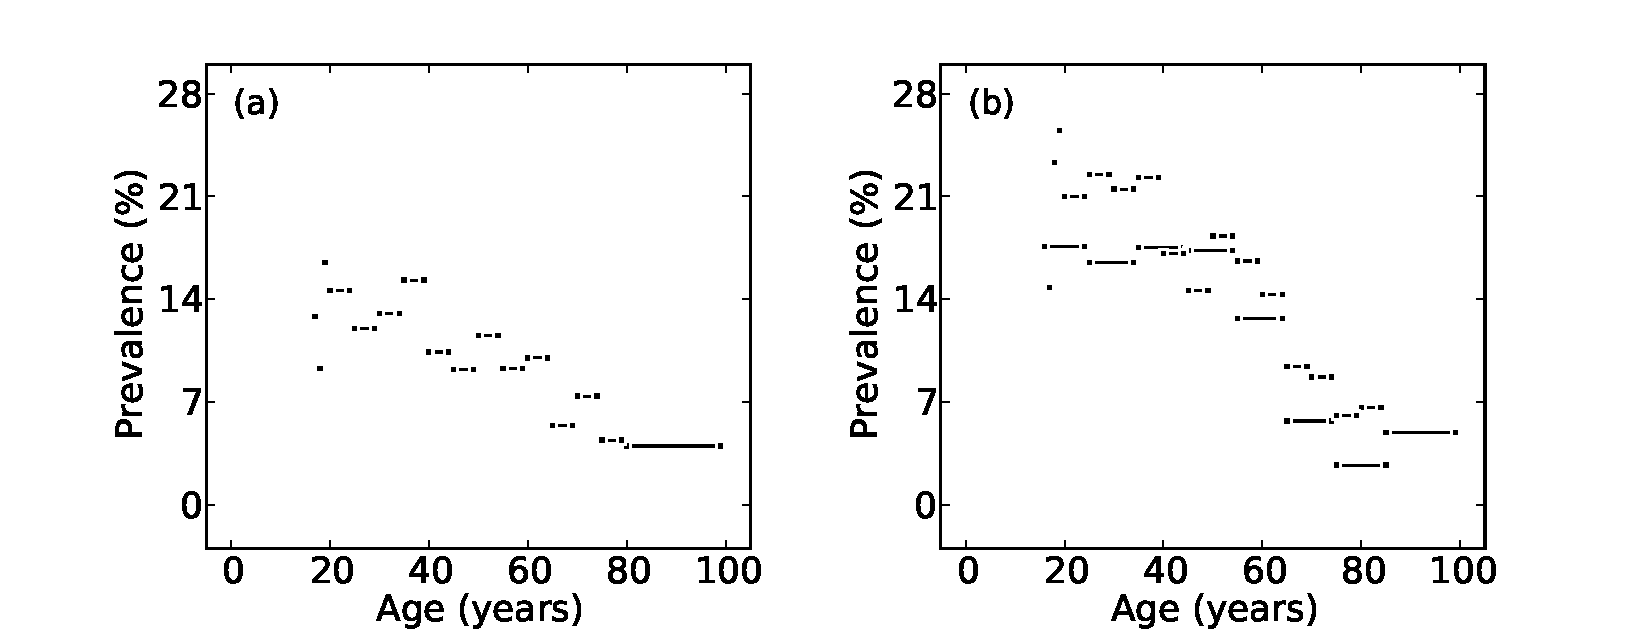
\includegraphics[width=\textwidth]{anxiety-data_by_cv.pdf}
            \caption{Point and period prevalence data for female anxiety disorders collected in systematic review for 2000-2010 in Australasia.}
            \label{fig:app-anxiety data}
        \end{center}
    \end{figure}

Excluding period prevalence measurements reduces the quantity of data and produces results that are generally much lower than estimates using all of the data without fixed effects.  Using a fixed effect study-level covariate allows the model to use all available data and explain the systematic bias and variation that results from different recall periods, as seen in Figure \ref{fig:app-anxiety FE}.

    \begin{figure}[h]
        \begin{center}
            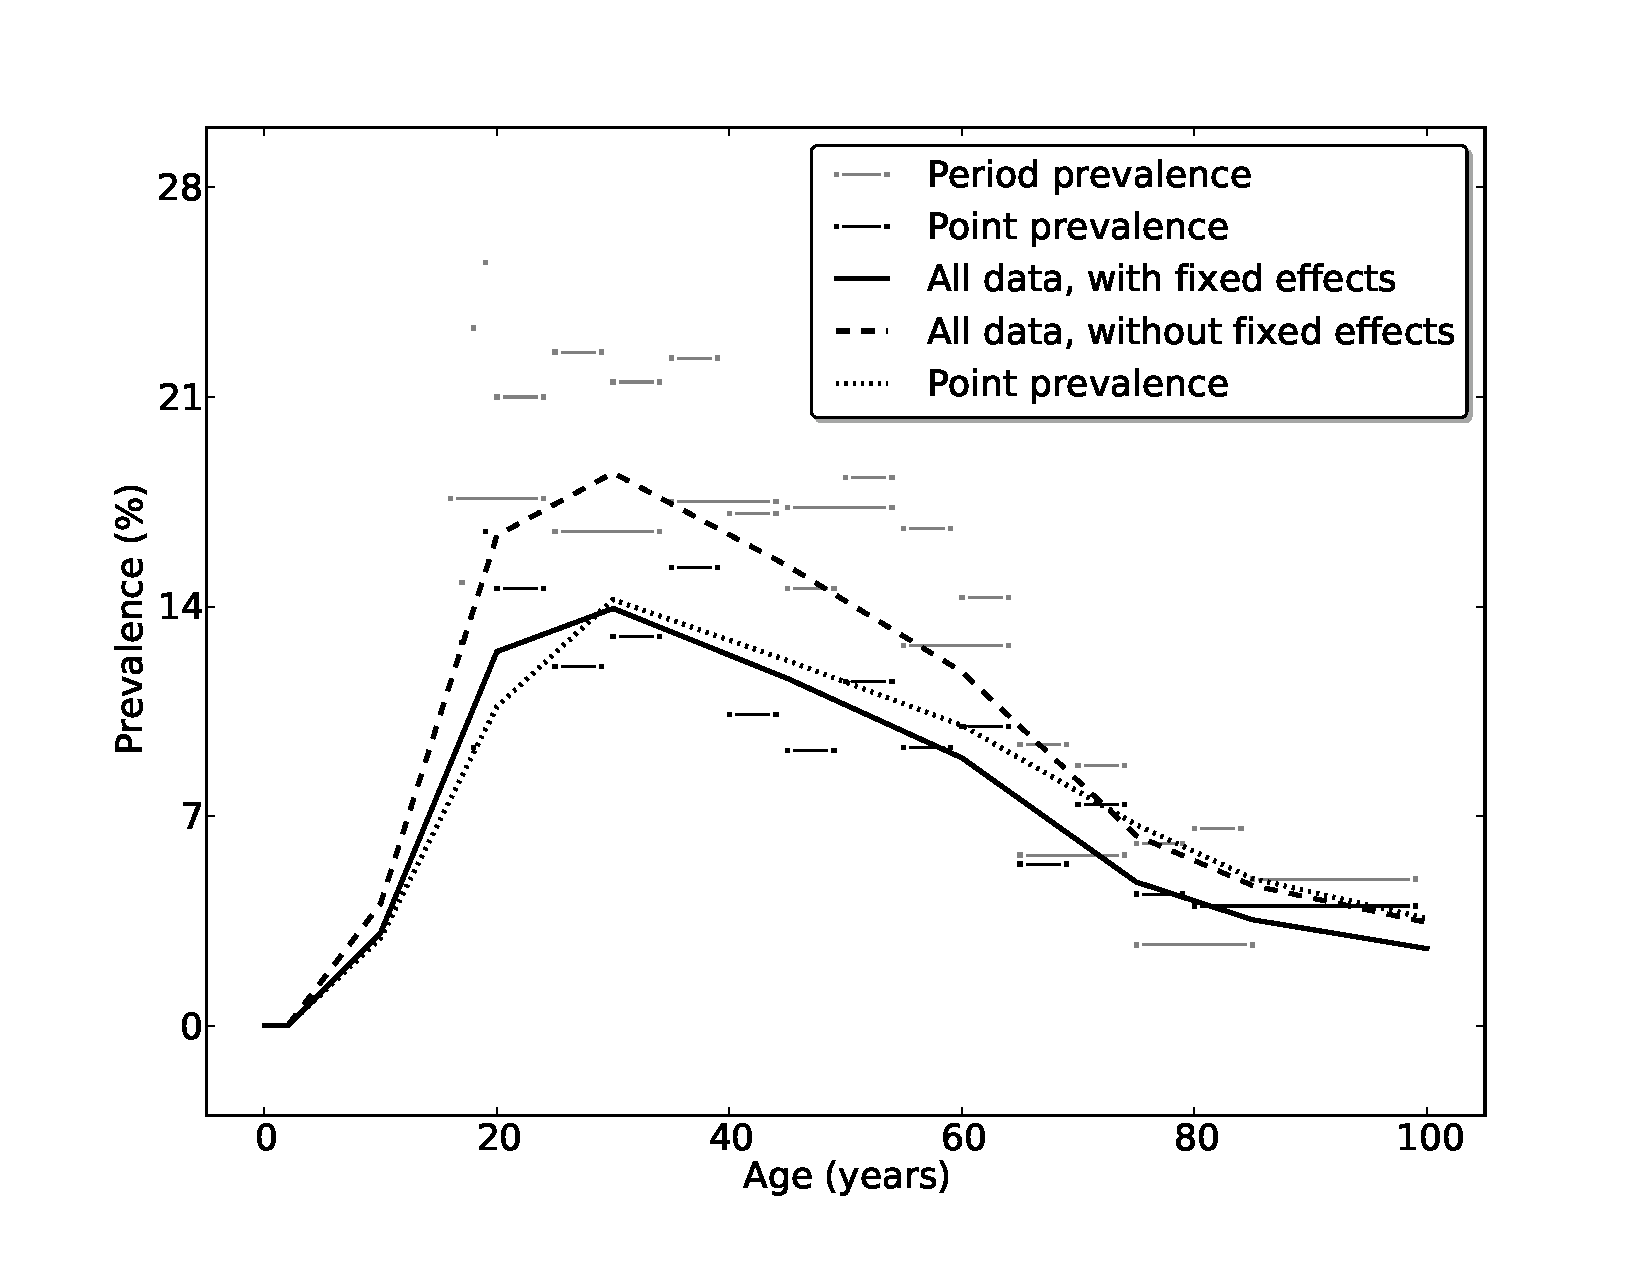
\includegraphics[width=\textwidth]{anxiety-FE.pdf}
            \caption{Comparison of prevalence estimates for anxiety disorders in 2005 for women in Australasia using point prevalence data only, point and period prevalence data with and without a fixed effect.}
            \label{fig:app-anxiety FE}
        \end{center}
    \end{figure}

